\documentclass[12pt, twoside]{article}
\usepackage[francais]{babel}
\usepackage[T1]{fontenc}
\usepackage[latin1]{inputenc}
\usepackage[left=1cm, right=1cm, top=8mm, bottom=8mm]{geometry}
\usepackage{float}
\usepackage{graphicx}
\usepackage{array}
\usepackage{multirow}
\usepackage{amsmath,amssymb,mathrsfs}
\usepackage{soul}
\pagestyle{empty}
\begin{document}


\section*{\center{Correction DM3}}

\subsection*{Exercice 2}

Soit $ABC$ un triangle �quilat�ral de c�t� $6$. On note $[CH]$ la hauteur du
triangle issue de $C$.
\medskip


\begin{tabular}{cc}
\begin{minipage}{5cm}
\begin{center}
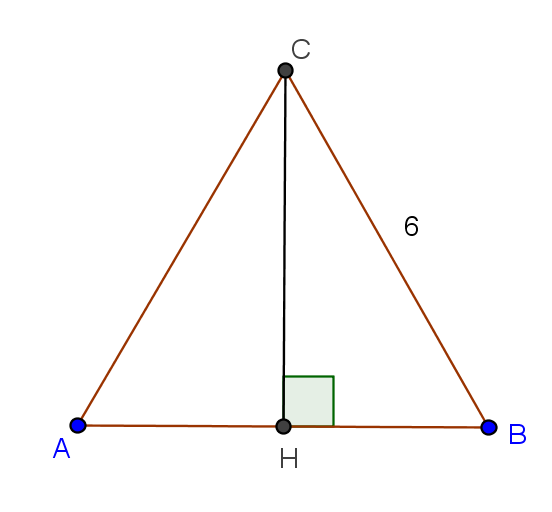
\includegraphics[width=5cm]{images/equi1.png}
\end{center}
\end{minipage}
&
\begin{minipage}{11cm}
\ul{M�thode 1}: 

\enskip

Comme $ABC$ est un triangle �quilat�ral, $(CH)$ est aussi la
m�diatrice de $[AB]$ donc $BH=\frac{AB}{2}=3$. Dans le triangle $CBH$
rectangle en $H$, j'utilise le th�or�me de Pythagore: \\
$BC^{2}=CH^{2}+BH^{2}$ d'o� $CH^{2}=BC^{2}-BH^{2}=6^{2}-3^{2}=27$. 

\enskip

d'o� \fbox{$CH=3\sqrt{3} \simeq 5,196$}

\end{minipage}
\end{tabular}

\medskip

\ul{M�thode 2}: 

\enskip

$\widehat{CBA}=\widehat{BAC}=\widehat{ACB}=60�$. Dans le triangle $CBH$
rectangle en $H$, on a : $\sin \widehat{CBH}=\dfrac{CH}{BC}$.

\enskip

Donc \fbox{$CH=6 \times \sin 60� \simeq 5,196$}


\bigskip



\begin{tabular}{cc}
\begin{minipage}{13cm}
\ul{FIGURE CLE}: Dans un triangle �quilat�ral de c�t� $a$, la hauteur $h$ est
donn�e par la formule:
\fbox{\textbf{$h=\dfrac{a}{2}\sqrt{3}$}}
\end{minipage}
&
\begin{minipage}{5cm}
\begin{center}
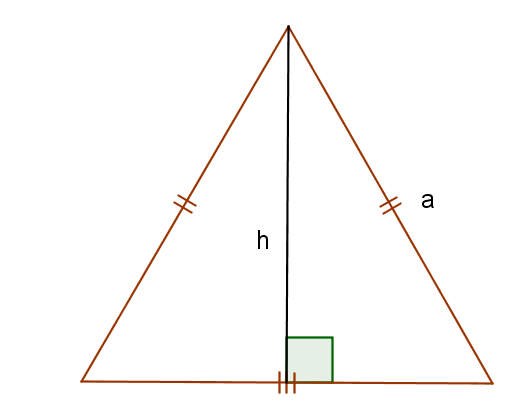
\includegraphics[width=4cm]{images/equi2.png}
\end{center}
\end{minipage}
\end{tabular}


\subsection*{Exercice 3}
\begin{enumerate}
  \item $31^{2}=(30+1)^{2}=30^{2}+ 2 \times 30+1=900+60+1=961$
  
  $81^{2}=(80+1)^{2}=80^{2}+ 2 \times 80+1=6400+160+1=6561$
  
  $59^{2}=(60-1)^{2}=60^{2}- 2 \times 60+1=3600-120+1=3481$ \\
 \ul{Autre m�thode}: 
  $59^{2}=(50+9)^{2}=50^{2}+ 2 \times 50 \times 9+9^{2}=2500+100 \times
  9+81=2500+900+81=3481$
  
  \enskip
  
  \item $A=899 \thinspace 999 \thinspace 999 \thinspace 999 \thinspace 999=9
  \times 10^{14}-1=(3\times 10^{7})^{2}-1^{2}=(3\times 10^{7}+1)(3\times
  10^{7}-1)$

  donc $A=30 \thinspace 000 \thinspace 001 \times 29 \thinspace 999
  \thinspace 999 $

 $30 \thinspace 000 \thinspace 001\neq1$, $30 \thinspace 000 \thinspace
 001\neq A$, et
 $30 \thinspace 000 \thinspace 001$ divise $A$ donc $899 \thinspace 999
 \thinspace 999 \thinspace 999 \thinspace 999$ n'est pas un nombre premier.
 
 \medskip
 
 Par la m�me m�thode, on montre que les autres nombres ne sont pas premiers (�
 compl�ter\ldots)
 
 \enskip
 
 $B=63 \thinspace 993 \thinspace 439= 64 \times 10^{6}-6561=(8 \times
 10^{3})^{2}-81^{2}=(8000-81)(8000+81)$
 
 \enskip
 
 $C=224 \thinspace 999  \thinspace 999 \thinspace 999 \thinspace 039=225 \times
 10^{12}-961=(15\times 10^{6})^{2}-31^{2}=(15\times 10^{6}+31)(15\times
 10^{6}-31)$
 
 \enskip
 
$D=899 \thinspace 999 \thinspace 999 \thinspace 996 \thinspace 519=9 \times
10^{14}-3481=(3 \times 10^{7})^{2}-59^{2}=(3\times 10^{7}+59)(3\times
10^{7}-59)$

\enskip

$E=1 \thinspace 599 \thinspace 999 \thinspace 999 \thinspace 999 \thinspace
559= 16\times 10^{14}-441=(4 \times 10^{7})^{2}-21^{2}=(4 \times 10^{7}+21)(4
\times 10^{7}-21)$
\end{enumerate}




\end{document}
